\chapter{THẢO LUẬN VÀ SO SÁNH}

\section{So sánh hai phương án tiền xử lý (Pipeline A vs Pipeline B)}
Kết quả thực nghiệm đã chứng minh rõ ràng vai trò tích cực của kỹ thuật tiền xử lý cải tiến:
\begin{itemize}
    \item Đối với KNN: Pipeline B nâng Accuracy từ $82.63\%$ lên $82.93\%$, Recall tăng từ $74.18\%$ lên $75.48\%$ và F1-Score tăng từ $75.98\%$ lên $76.61\%$. Việc gom nhóm các quốc gia hiếm giúp giảm độ phân tán của không gian khoảng cách Euclid, trong khi chuẩn hóa \texttt{RobustScaler} làm giảm tác động của các giá trị ngoại lệ trong biến \texttt{lead\_time}.
    \item Đối với Decision Tree: Các đặc trưng phái sinh như \texttt{room\_type\_changed} (phòng bị đổi có tỷ lệ hủy chỉ $5.45\%$) và \texttt{is\_family} đã trở thành các điểm phân tách cực kỳ hữu ích ở các tầng trên cùng của cây quyết định.
\end{itemize}

\section{So sánh thuật toán KNN và Decision Tree}
\begin{itemize}
    \item \textbf{Về mặt hiệu năng:} Decision Tree vượt trội hoàn toàn so với KNN ở mọi chỉ số (F1-score $80.12\%$ so với $76.61\%$, ROC-AUC $0.9289$ so với $0.8965$).
    \item \textbf{Về chi phí tính toán:} Decision Tree có tốc độ huấn luyện và dự đoán rất nhanh ($O(d \cdot \text{depth})$ khi dự đoán), trong khi KNN đòi hỏi tính toán khoảng cách tới hàng chục nghìn điểm huấn luyện nên tốn thời gian và bộ nhớ hơn đáng kể.
    \item \textbf{Về khả năng giải thích (Interpretability):} Cây quyết định cung cấp cấu trúc quy tắc phân nhánh \textit{if-else} trực quan, giúp nhà quản trị khách sạn hiểu được lý do tại sao một đơn phòng bị dự đoán có nguy cơ hủy cao.
\end{itemize}

\section{Phân tích tương quan giữa Precision, Recall và F1-score}
Trong bài toán quản trị khách sạn, có một sự đánh đổi (Trade-off) rõ rệt giữa Precision và Recall:
\begin{itemize}
    \item \textbf{EXP03 (Cây quyết định tiêu chuẩn):} Đạt Precision cao ($82.16\%$) nhưng Recall chỉ đạt $74.02\%$. Khi mô hình cảnh báo hủy, độ tin cậy rất cao (ít báo động giả), nhưng lại bỏ sót tới 2,298 đơn đặt phòng bị hủy (False Negative).
    \item \textbf{EXP05 (Cây quyết định Balanced):} Khi điều chỉnh trọng số phạt mẫu hủy, Recall tăng vọt lên $82.44\%$ (giảm số đơn bỏ sót xuống chỉ còn 1,553 đơn), nhưng kéo theo Precision giảm xuống $76.87\%$.
    \item Tùy thuộc vào chính sách kinh doanh (mùa cao điểm hay mùa thấp điểm), khách sạn có thể lựa chọn mô hình thiên về Recall (để chuẩn bị phòng bán lại) hoặc thiên về Precision (để tránh làm phiền khách hàng thực sự đến ở).

\end{itemize}

\section{Phân tích chuyên sâu về False Positive (Báo động giả)}
Nhóm False Positive (1,611 mẫu, chiếm $6.75\%$ tập test) là những đơn phòng được mô hình dự đoán sẽ hủy, nhưng thực tế khách vẫn đến nhận phòng (Check-Out thành công).
\begin{itemize}
    \item \textbf{Nguyên nhân:} Các đơn này thường có thời gian đặt trước rất dài (\texttt{lead\_time} lớn), không có yêu cầu đặc biệt và đi theo hình thức đặt qua đại lý trực tuyến (Online TA) -- vốn là các đặc điểm trùng khớp với các mẫu đơn bị hủy thông thường.
    \item \textbf{Rủi ro nghiệp vụ:} Nếu khách sạn tự động bán chồng phòng (Overbooking) quá sớm đối với nhóm này, khi khách đến nhận phòng khách sạn sẽ rơi vào tình trạng thiếu phòng và phải chịu chi phí bồi thường đắt đỏ.
\end{itemize}

\section{Phân tích chuyên sâu về False Negative (Bỏ sót rủi ro)}
Nhóm False Negative (1,857 mẫu, chiếm $7.78\%$ tập test) là những đơn phòng mô hình dự đoán sẽ không hủy, nhưng thực tế khách đã hủy phòng đột xuất.
\begin{itemize}
    \item \textbf{Đặc điểm thống kê:}
    \begin{itemize}
        \item Thời gian đặt trước (\texttt{lead\_time}) rất ngắn: Trung bình chỉ \textbf{83.40 ngày}, so với \textbf{161.89 ngày} của nhóm True Positive (nhóm bắt trúng hủy phòng).
        \item $75.82\%$ ca False Negative xảy ra tại \textbf{City Hotel} (khách sạn nội đô).
    \end{itemize}
    \item \textbf{Nguyên nhân nghiệp vụ:} Khách công vụ hoặc khách lưu trú ngắn hạn tại thành phố thường đặt phòng sát ngày và hủy phòng đột xuất do lịch trình làm việc thay đổi vào phút chót. Hành vi này không để lại dấu hiệu cảnh báo trước trong dữ liệu đặt phòng ban đầu.
\end{itemize}

\begin{figure}[H]
    \centering
    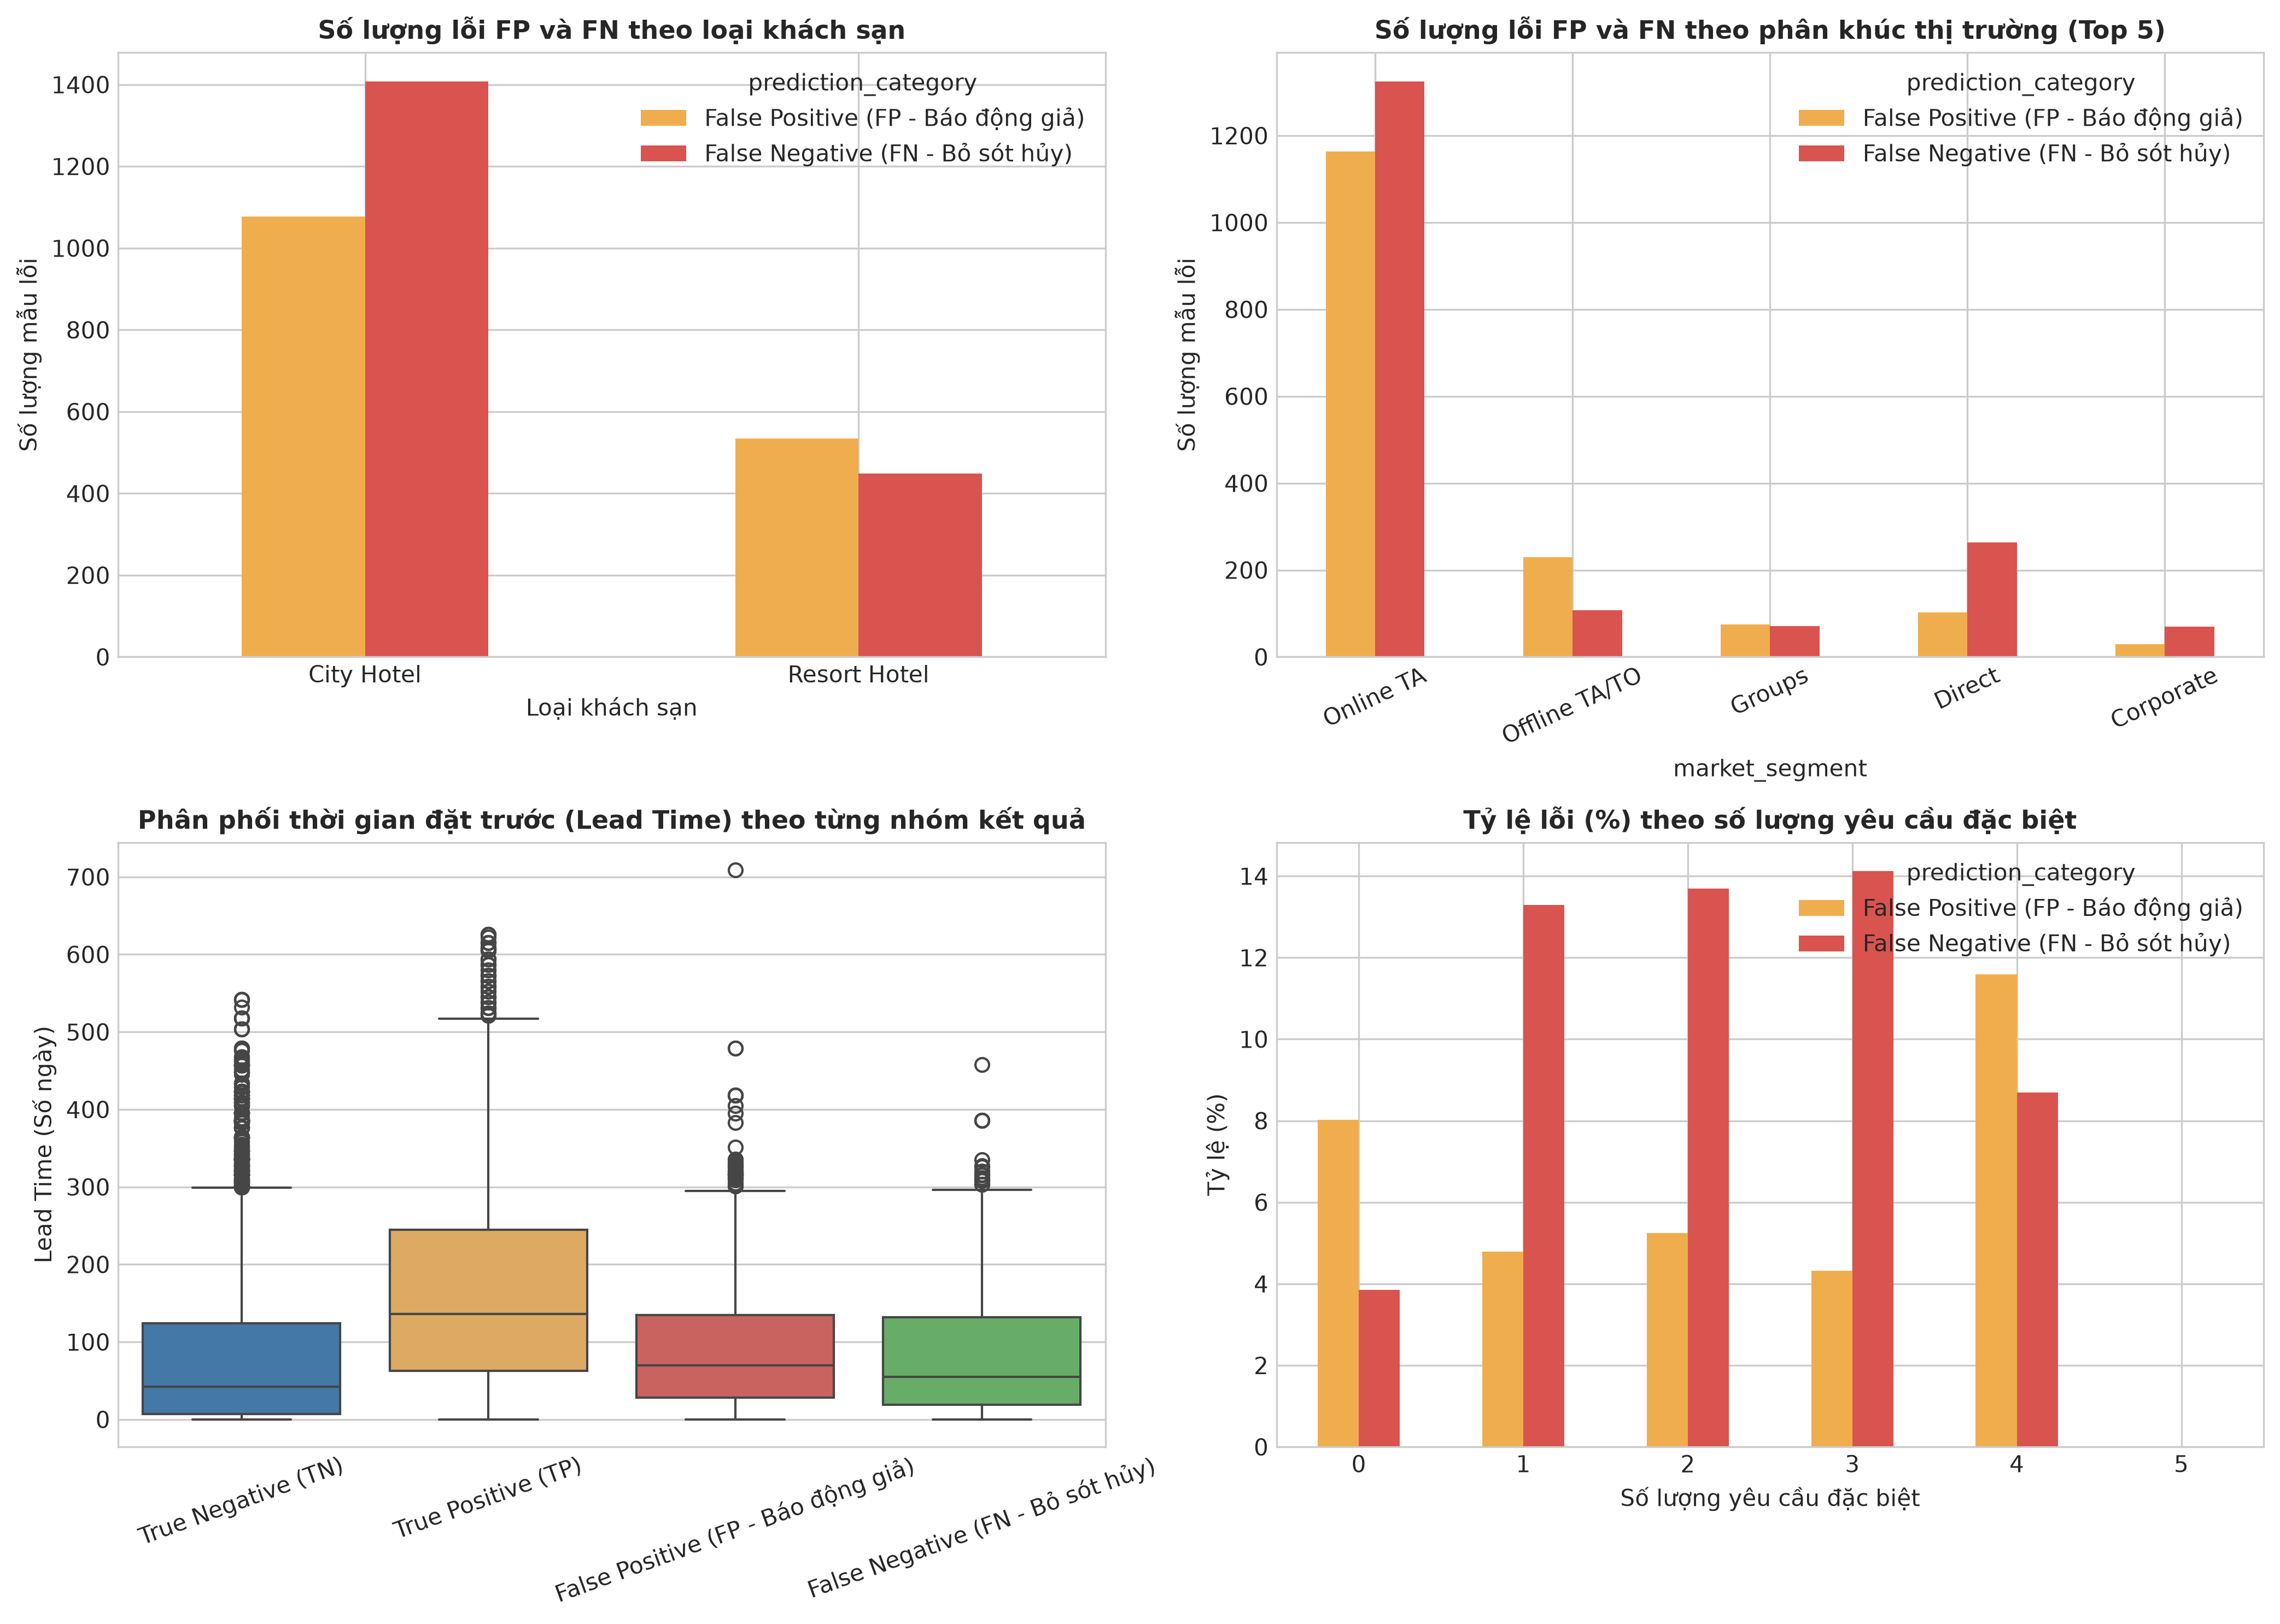
\includegraphics[width=0.9\linewidth]{error_analysis_breakdown.png}
    \caption{Phân bố lỗi False Positive và False Negative theo các đặc trưng nghiệp vụ}
    \label{fig:error_breakdown}
\end{figure}

\section{Hạn chế của dữ liệu và mô hình}
\begin{itemize}
    \item \textbf{Thiếu thông tin kinh tế vĩ mô và thời tiết:} Dữ liệu chưa tích hợp giá vé máy bay, yếu tố thời tiết hoặc các sự kiện lễ hội tại địa phương.
    \item \textbf{Dữ liệu ẩn danh:} Không có mã định danh khách hàng duy nhất để phân tích hành vi lịch sử dài hạn của từng cá nhân (Customer Lifetime Behavior).
    \item \textbf{Đặc thù thuật toán KNN:} KNN không phù hợp cho các hệ thống phục vụ trực tuyến quy mô lớn do chi phí bộ nhớ và độ trễ truy vấn cao.
\end{itemize}

\section{Khả năng ứng dụng thực tế trong quản trị khách sạn}
Mô hình tối ưu EXP06 có thể được tích hợp trực tiếp vào hệ thống Quản lý tài sản khách sạn (Property Management System -- PMS):
\begin{enumerate}
    \item \textbf{Định lượng tỷ lệ Overbooking động:} Dự báo chính xác số lượng phòng có nguy cơ bị hủy để khách sạn chủ động mở bán vượt mức tương ứng mà không sợ thiếu phòng.
    \item \textbf{Chính sách chăm sóc khách hàng chủ động:} Với các đơn đặt trước từ 3 tháng trở lên được cảnh báo có nguy cơ hủy, bộ phận lễ tân có thể gửi email xác nhận lịch trình, đề xuất giảm giá bữa ăn hoặc dịch vụ đưa đón để giữ chân khách hàng.
\end{enumerate}
